    \documentclass[10pt]{beamer}
    

    %% Compile using xelatex --
    %% Then biber lecture6
    %% Then xelatex again
    \usetheme{glasgow}
    
    \usepackage{booktabs}
    \usepackage[scale=2]{ccicons}
    \usepackage{minted}
    \usepackage{bookmark}
    \usepackage[style=verbose,backend=biber]{biblatex}
    \usepackage{filecontents}% to embed the file `myreferences.bib` in your `.tex` file
    % \begin{filecontents*}{refs.bib}
    %     @misc{schneider_understanding_nodate,
    %     title = {Understanding the {FDTD} {Method}},
    %     url = {https://eecs.wsu.edu/~schneidj/ufdtd/},
    %     author = {Schneider, John}
    % }
    % \end{filecontents*}

    \addbibresource{refs.bib}

    % \usepackage[noadjust]{cite}
    \usepgfplotslibrary{dateplot}
    
    \usemintedstyle{trac}
    
    % ($ (A)!r!(B) $) the location of images to be used
    \graphicspath{{src/}}
    
    %% Customisation
    % \newcommand{\V}[1]{\v} % vectors \v{c}
    % \renewcommand{\v}[1]{\mathbf{#1}} % vectors
    \newcommand{\ti}[1]{\tilde{#1}} % spectral representation
    \newcommand{\tnsr}[1]{\underline{\underline{#1}}}
    
    % Symbols
    \renewcommand{\O}{\omega}  % omega
    \newcommand{\E}{\varepsilon}  % epsilon
    \renewcommand{\u}{\mu}  % mu
    \newcommand{\p}{\rho}  % rho
    \newcommand{\x}{\times}  % times
    \renewcommand{\inf}{\infty}  % infinity
    \newcommand{\infint}{\int\limits_{-\inf}^\inf} % integral by R
    \newcommand{\e}{\mathrm{e}} % Straight-up exponential
    \renewcommand{\j}{{j}\mkern1mu} % Straight-up exponential
    \newcommand{\iu}{\mathrm{i}\mkern1mu}
    
    \newcommand\ddfrac[2]{\frac{\displaystyle #1}{\displaystyle #2}}
    
    \usepackage{animate}
% Define a the counter cnt. Used to identify files generated for use
% with Gnuplot.
\newcounter{cnt}
\setcounter{cnt}{0}

% Macro for drawing one frame of the F-distribution animation.
\newcommand{\fdst}[4]{%
    % shade the critical region tail
    \draw[fill,orange]  (#1,0) -- plot[id=5\thecnt,domain=#1:5.5,samples=50]
        function {#4*(x**(0.5*#2-1))*((1+#2*x/#3)**(-0.5*#2-0.5*#3))}
            -- (5.5,0) -- cycle;

    % draw the F distribution curve
    \draw[color=blue!50!black,thick]
        plot[id=f4\thecnt,smooth,domain=0:5.5,samples=100]
        function {#4*(x**(0.5*#2-1))*((1+#2*x/#3)**(-0.5*#2-0.5*#3))};

    % draw the F axis
    \draw[->] (0,0) -- (6,0) node[right] {$F$};
    % label the critical region boundary
    \draw (#1,0) -- (#1,-0.02) node[below] {$#1$};
    % label 0
    \draw (0,0) -- (0,-0.02) node[below] {$0$};

    % add some lables for degrees of freedom and alpha level
    \draw (2,0.5) node[right] {$df_1 = #2$};
    \draw (2,0.4) node[right] {$df_2 = #3$};
    \draw (2,0.3) node[right] {$\alpha = 0.10$};

    % draw the y axis
    \draw[very thin,->] (0,0) -- (0,0.8);
}


    \title{High Frequency Communication Systems}
    \subtitle{Lecture 6}
    \date{Spring 2022}
    \author{Hasan T Abbas \& Qammer H Abbasi}
    % \institute{}
    




\begin{document}

\maketitle

%%%%%%%%%%%%%%%%%%%%%%%%%%%%%%%%%%%%%%%%%%
%%%%%%%%%%%%%%%%%%%%%%%%%%%%%%%%%%%%%%%%%%
%%%%%%%%%%%%%%%%%%%%%%%%%%%%%%%%%%%%%%%%%%
\begin{frame}[fragile]
    \frametitle{Lecture Outline}
    \begin{outline}[itemize]
        \1 Numerical Methods in Electromagnetics
        \1 Discretisation of Maxwell's Equations
        \1 Finite Difference Time Domain method
    \end{outline}
\end{frame}
%%%%%%%%%%%%%%%%%%%%%%%%%%%%%%%%%%%%%%%%%%
%%%%%%%%%%%%%%%%%%%%%%%%%%%%%%%%%%%%%%%%%%
%%%%%%%%%%%%%%%%%%%%%%%%%%%%%%%%%%%%%%%%%%

\section{Numerical Methods in Electromagnetics}




\begin{frame}
    \frametitle{Electromagnetic Simulation Methods}
    \begin{outline}
        \1 There are many numerical methods developed to solve Maxwell's or wave equations
    \end{outline}
    \begin{figure}[h!]
        \centering
        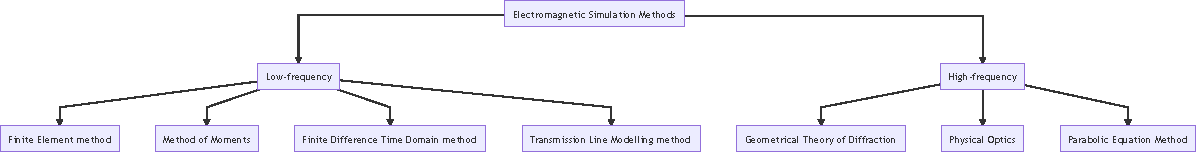
\includegraphics[width=1.0\textwidth]{em methods_1.pdf}
        \caption{Various simulation methods in EM}
    \end{figure}
\end{frame}

\begin{frame}
    \frametitle{Frequency Domain Methods}
    \begin{columns}[T] % align columns
        \begin{column}{.6\textwidth}
            \begin{outline}
                \1 We solve either a differential or integral equation \textit{numerically}
                \2 Only at a single frequency
                \1 These methods are relatively more accurate than time domain methods
                \2 However, mathematically they are more complex
                \1 Finite element method (FEM) is the most computational tool used in all areas of engineering including electromagnetic simulation (e.g. HFSS, CST and COMSOL)
                \2 It solves partial differential equations by discretisation into \textit{finite elements}
            \end{outline}
        \end{column}
        \begin{column}{.4\textwidth}
            \begin{figure}[B!]
                \centering
                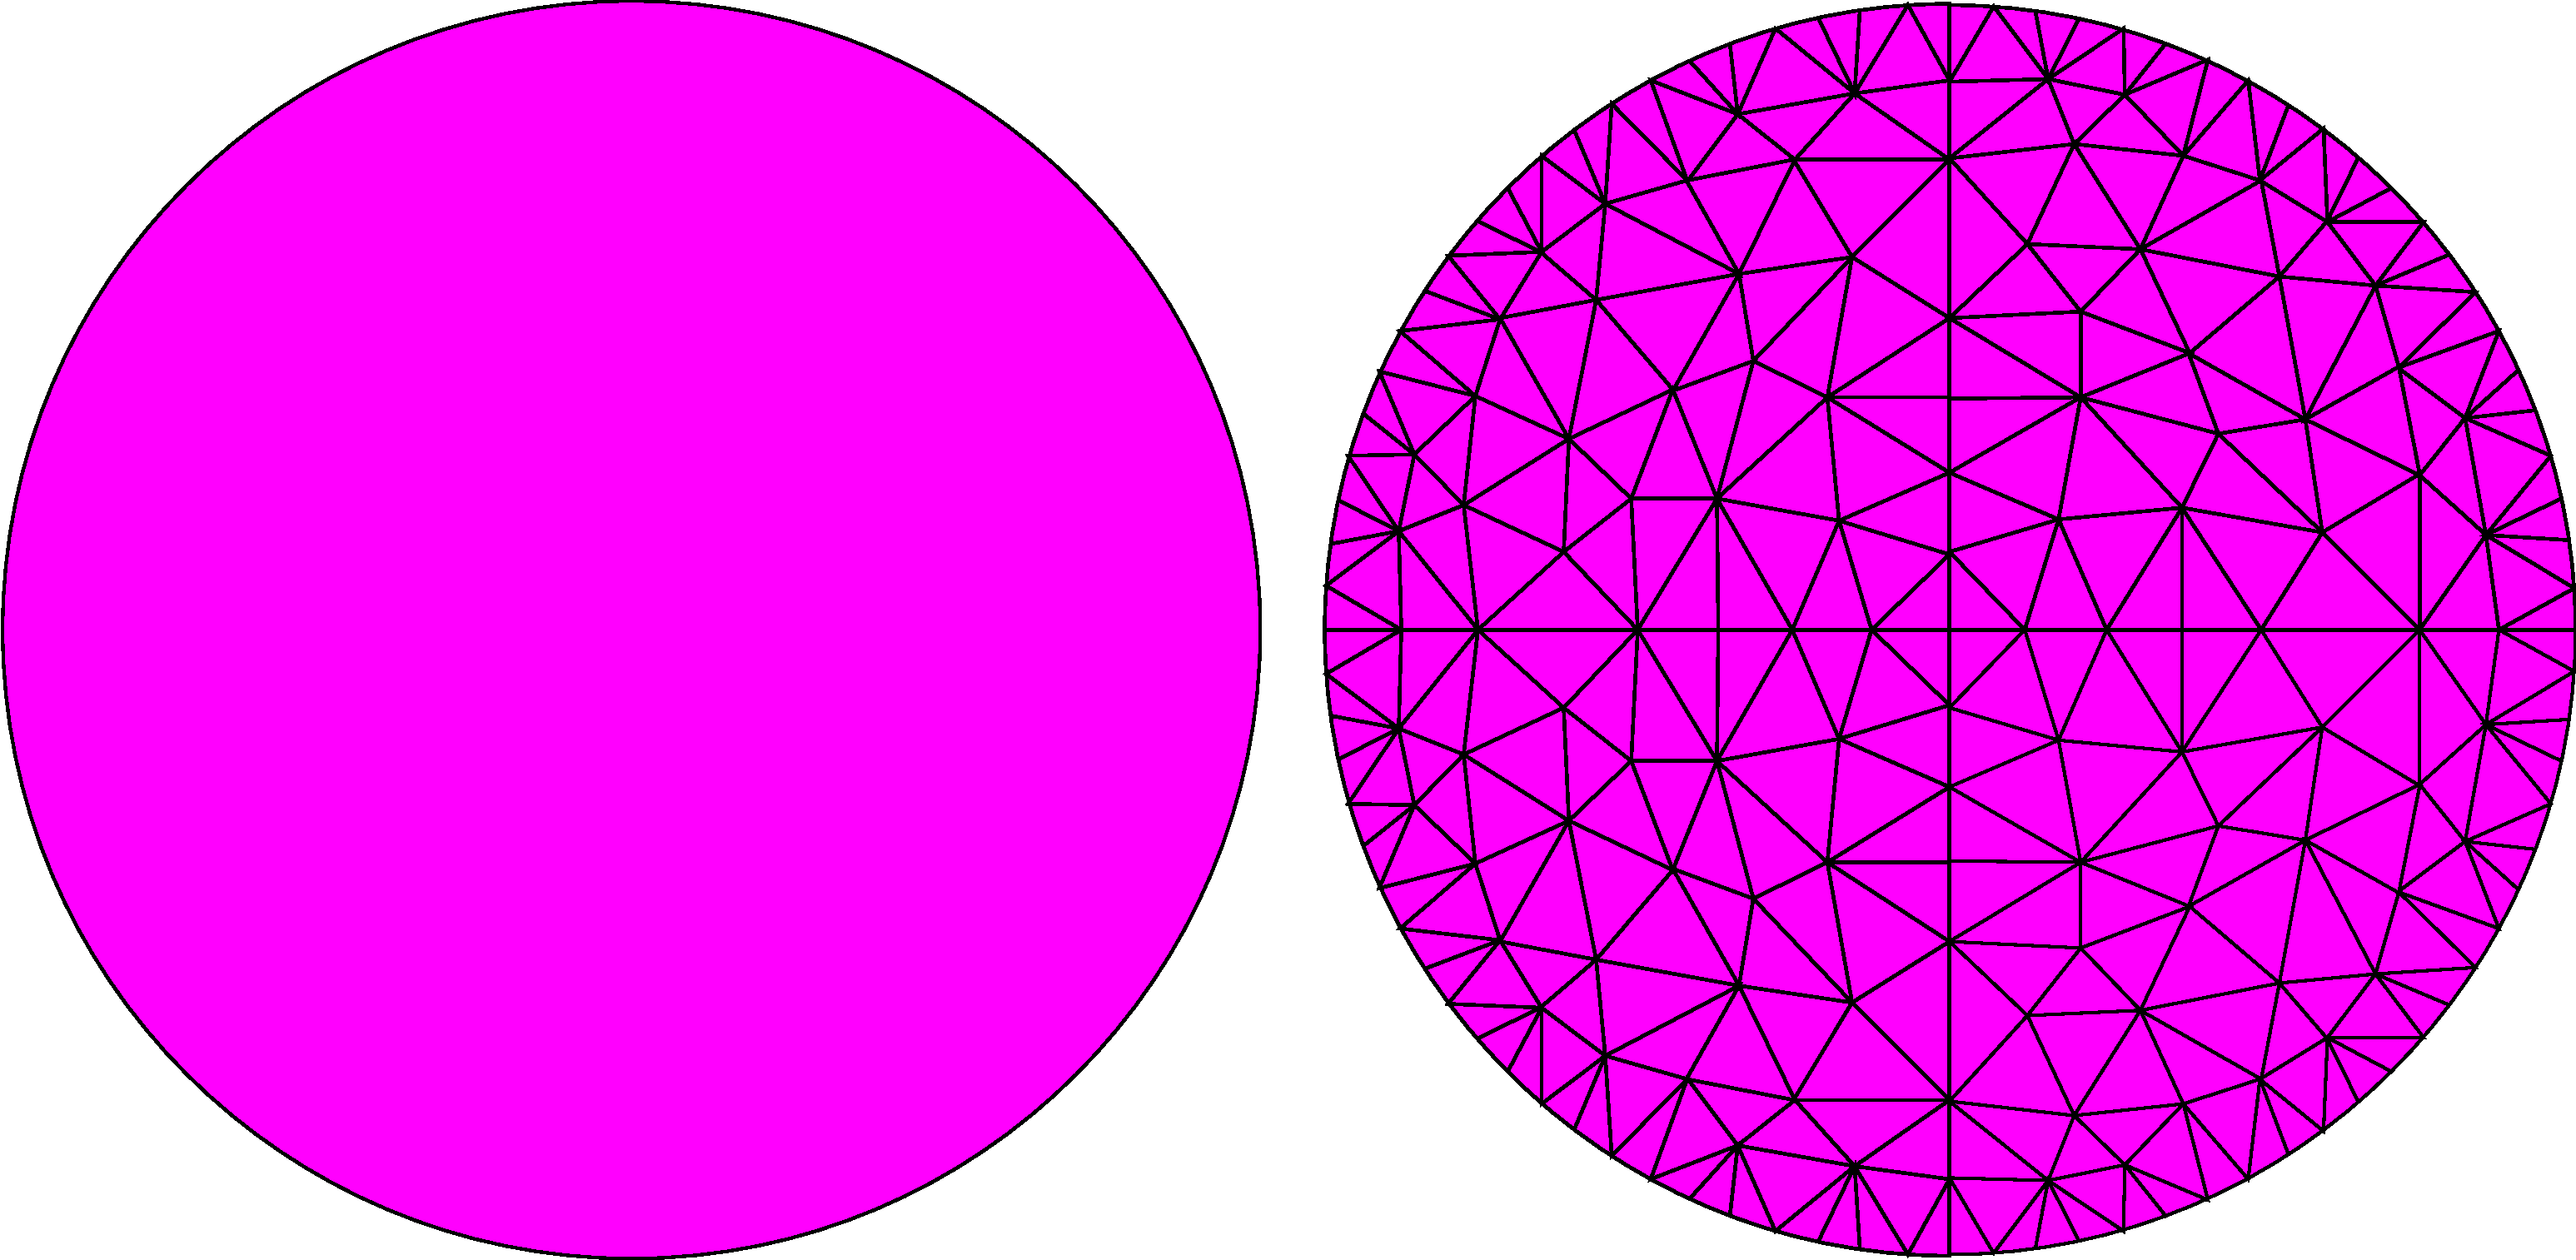
\includegraphics[width=1\textwidth]{mesh.pdf}
                \caption{Typical mesh in FEM}
            \end{figure}
        \end{column}%
    \end{columns}

\end{frame}

\begin{frame}
    \frametitle{Time Domain Methods}


    \begin{columns}[T] % align columns
        \begin{column}{.6\textwidth}
            \begin{outline}
                \1 We observe the numerical time evolution of electromagnetic fields or currents through a region of space
                \1 They are more intuitive as we can \textit{visualise} wave phenomena
                \1 We can obtain all the frequency information in one run through the Fourier transformation
                \1 Simplicity comes at the cost of problems such as numerical stability and dispersion
                \1 However, we will look into the finite difference time domain (FDTD) method deeply
            \end{outline}
        \end{column}
        \begin{column}{.4\textwidth}
            \begin{figure}[B!]
                \centering
                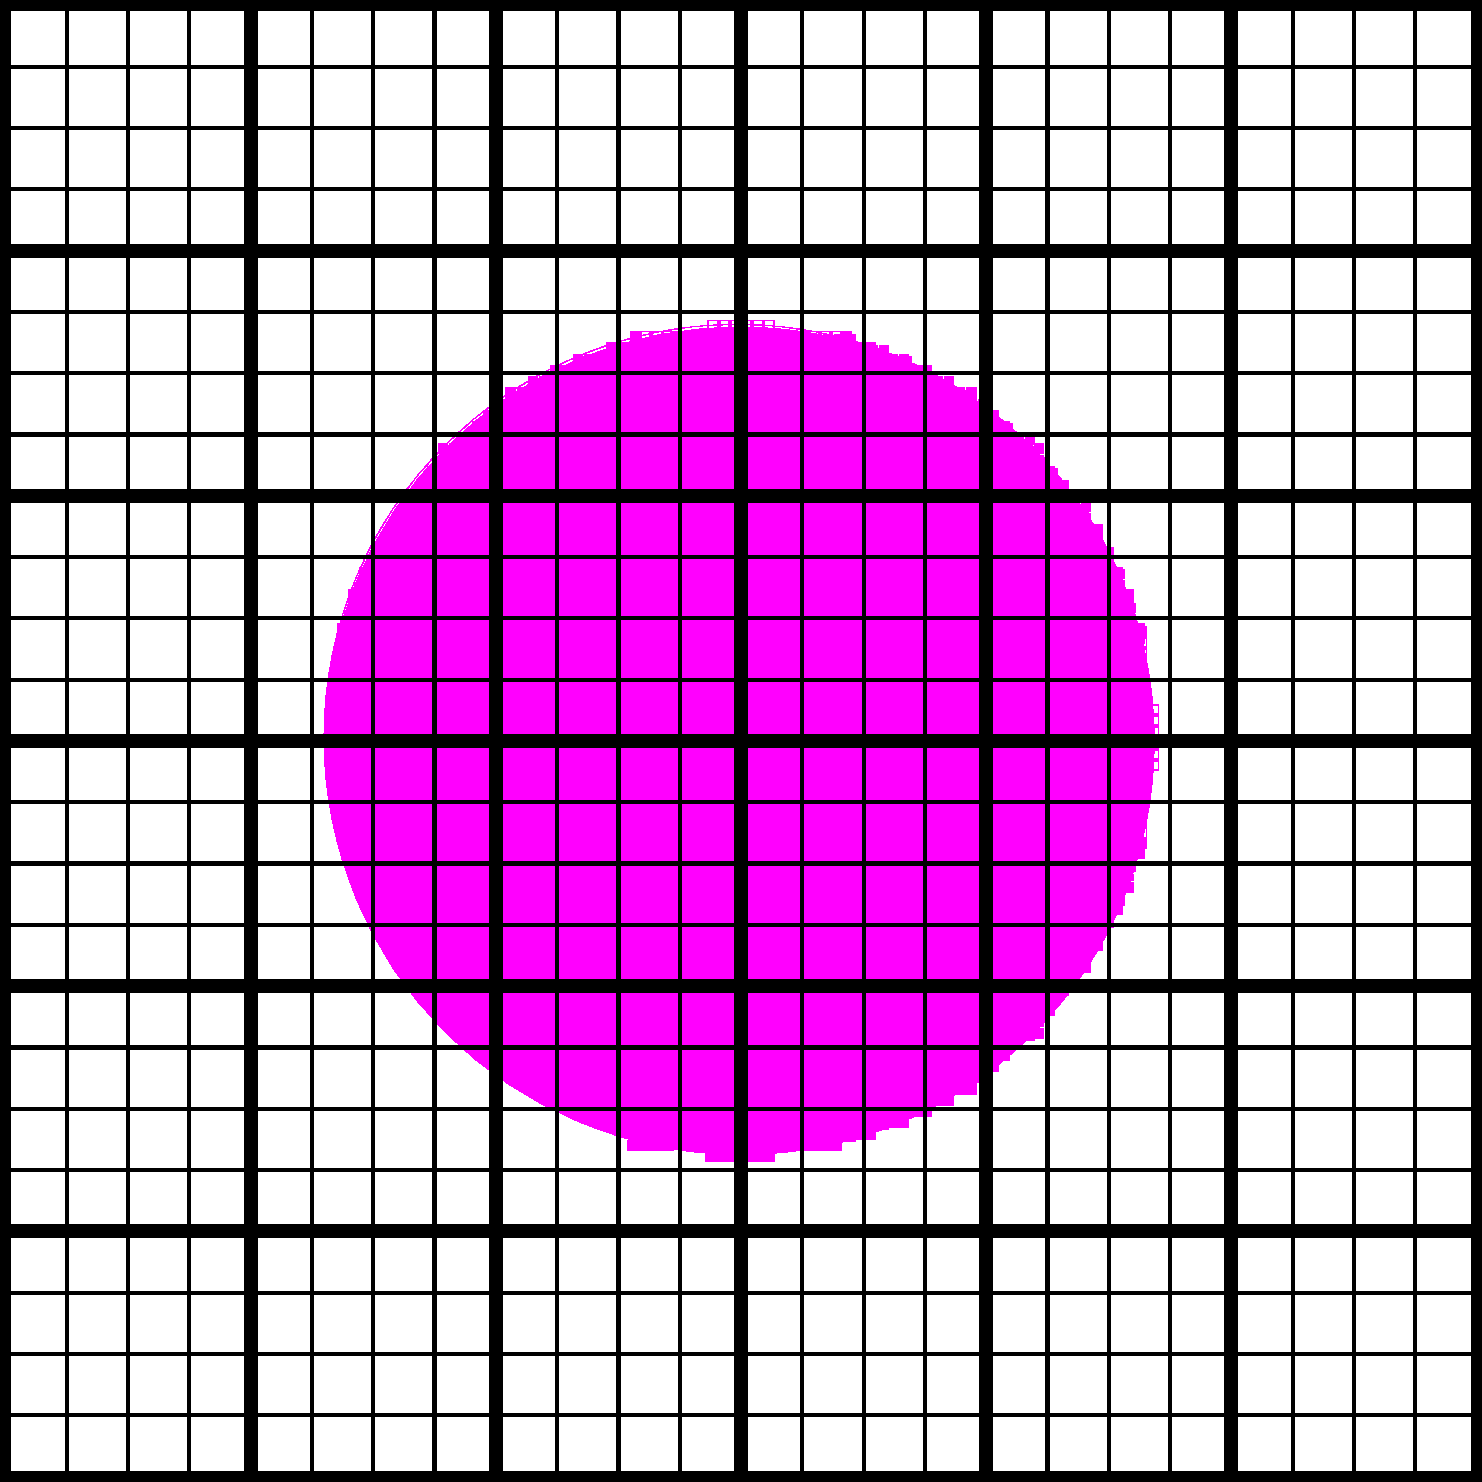
\includegraphics[width=1\textwidth]{fdtd mesh.pdf}
                \caption{Typical mesh in FDTD}
            \end{figure}
        \end{column}%
    \end{columns}
\end{frame}

\section{Finite Difference Method}
\begin{frame}
    \frametitle{Solving differential equations}
    \begin{outline}
        \1 The goal is to solve differential equations \textit{numerically} given some initial and boundary conditions
        \1 Maxwell's equations has operators such as curl $\curl$, divergence $\div$, and Laplacian $\laplacian$
        \1 Lets first express the derivative term as a difference formula.
    \end{outline}

\end{frame}

\begin{frame}
    \frametitle{The Discretisation Process}

    \begin{outline}
        \1 We aim to \textcolor{red}{transform} a Calculus problem into a linear algebra one
        \1 In other words, through discretisation, we move from the continuous domain to the discrete domain
        \1 A partial differential equation is thus converted into a difference equation
    \end{outline}
    \begin{figure}[htbp]
        \centering
        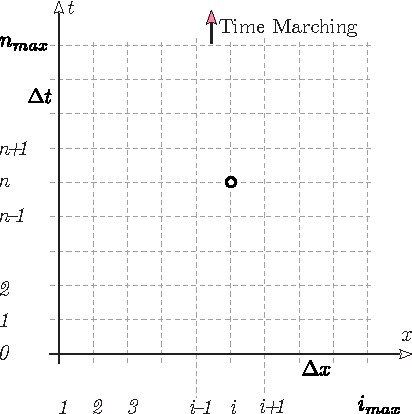
\includegraphics[width=.45\textwidth]{time_marching.pdf}

    \end{figure}

\end{frame}

\begin{frame}
    \frametitle{Central Differencing}
    Consider the Taylor series expansions of the function $f(x)$ expanded about the
    point $x_0$ with an offset of $\pm\Delta/2$:

    \begin{align*}
        f(x_0 + \frac{\Delta}{2}) & = f(x_0) + \frac{\Delta}{2} f'(x_0) +
        \frac{1}{2!}\left(\frac{\Delta}{2}\right)^2 f''(x_0) +
        \frac{1}{3!}\left(\frac{\Delta}{2}\right)^3 f'''(x_0) + \ldots,   \\
        f(x_0 - \frac{\Delta}{2}) & = f(x_0) - \frac{\Delta}{2} f'(x_0) +
        \frac{1}{2!}\left(\frac{\Delta}{2}\right)^2 f''(x_0) -
        \frac{1}{3!}\left(\frac{\Delta}{2}\right)^3 f'''(x_0) + \ldots
    \end{align*}

    here the primes indicate differentiation. Subtracting the second equation from the first yields,
    \begin{equation}
        f\left(x_0+\frac{\Delta}{2}\right) -
        f\left(x_0-\frac{\Delta}{2}\right) =
        \Delta f'(x_0) +
        \frac{2}{3!}\left(\frac{\Delta}{2}\right)^3 f'''(x_0) + \ldots
        \label{eq:diff}
    \end{equation}
\end{frame}

\begin{frame}
    \frametitle{Central Difference Formula for Derivatives}

    Moving on and dividing Eq. \ref{eq:diff} by $\Delta$ we get,

    \begin{equation*}
        \frac {f\left(x_0 + \frac{\Delta}{2}\right) -
            f\left(x_0 - \frac{\Delta}{2}\right)}{\Delta} =  f'(x_0) + \frac{1}{3!}\frac{\Delta^2}{2^2} f'''(x_0) + \ldots
    \end{equation*}
    The term on the left is the derivative term of the $f(x)$ at point $x_0$ plus an approximation term, $O(\Delta^2)$:
    \begin{equation*}
        \dv{f}{x}|_{x=x_0} = \frac{f\left(x_0+\frac{\Delta}{2}\right) -f\left(x_0-\frac{\Delta}{2}\right)}{\Delta} + O(\Delta^2).
    \end{equation*}

    The central difference formula is thus:
    \begin{tcolorbox}[colback=blue!5,colframe=university-blue]
        \begin{equation*}
            \dv{f}{x}|_{x=x_0} \approx \frac{f\left(x_0+\frac{\Delta}{2}\right) -
                f\left(x_0-\frac{\Delta}{2}\right)}{\Delta}.
        \end{equation*}
    \end{tcolorbox}
\end{frame}

\begin{frame}
    \frametitle{The Divergence Operator}

    % \mqty[\vu{x} & \vu{y} & \vu{z} \\ \pdv{x} & \pdv{y} & \pdv{z} \\ E_{x} & E_{y} & E_{z}] 
    \begin{columns}[T] % align columns
        \begin{column}{.6\textwidth}
            The divergence of a vector gives us a scalar field, and according to the Maxwell's equation:
            \begin{align*}
                \div{E} & = \frac{\rho}{\E} = \pdv{E_x}{x} + \pdv{E_y}{y} +\pdv{E_z}{z}
            \end{align*}
            For a 2D case, the above expression can be written as:
        \end{column}
        \begin{column}{.4\textwidth}
            \begin{figure}[T!]
                \centering
                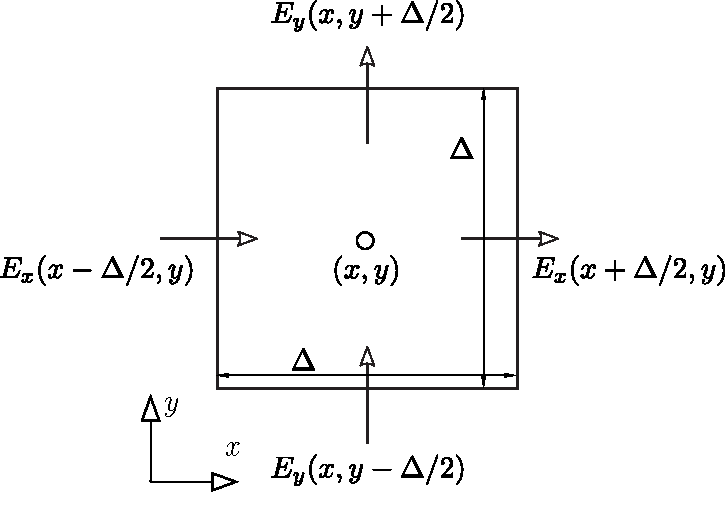
\includegraphics[width=.95\textwidth]{div_E.pdf}
            \end{figure}
        \end{column}%
    \end{columns}
    \small
    \begin{align*}
        \pdv{E_x}{x} + \pdv{E_y}{y} \approx \frac{\left(E_{x}(x+\Delta/2, y) - E_{x} (x-\Delta/2, y) + E_{y} (x, y+\Delta/2) - E_{y}(x, y-{\Delta}/{2})\right)}{\Delta}
    \end{align*}

\end{frame}



\begin{frame}
    \frametitle{The Curl Operator}

    \begin{columns}[T] % align columns
        \begin{column}{.6\textwidth}
            Likewise, we use the curl $\curl$ operator in Maxwell's equations:
            \begin{align*}
                \curl{E} & = \mqty[\vu{x} & \vu{y} & \vu{z} \\ \pdv{x} & \pdv{y} & \pdv{z} \\ E_{x} & E_{y} & E_{z}]
            \end{align*}
            For a 2D case, the above expression can be written as:
        \end{column}
        \begin{column}{.4\textwidth}
            \begin{figure}[T!]
                \centering
                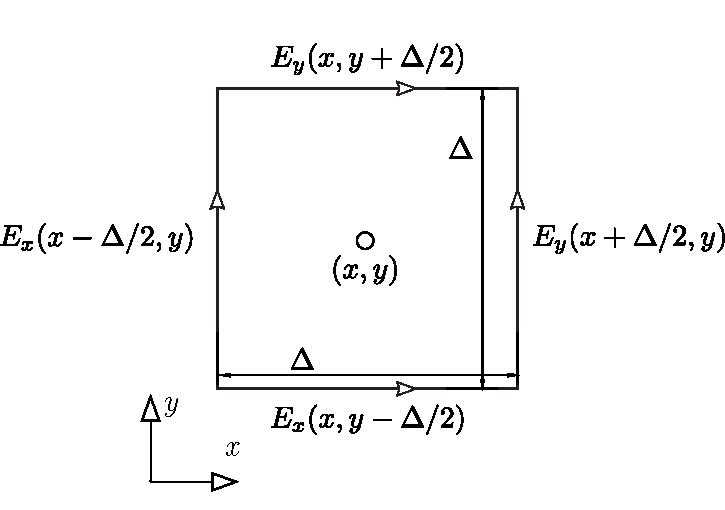
\includegraphics[width=.95\textwidth]{curl_E.pdf}
            \end{figure}
        \end{column}%
    \end{columns}
    \small
    \begin{align*}
        \pdv{E_y}{x} - \pdv{E_x}{y} \approx \frac{\left(E_{y}(x+\Delta/2, y) - E_{y} (x-\Delta/2, y) - E_{x} (x, y+\Delta/2) + E_{x}(x, y-{\Delta}/{2})\right)}{\Delta}
    \end{align*}
\end{frame}


\begin{frame}
    \frametitle{The Laplacian Operator}

    The wave equation possesses the $\laplacian$ operator:
    \begin{align*}
        \laplacian{\phi} & = \pdv[2]{\phi_x}{x} + \pdv[2]{\phi_y}{y} +  \pdv[2]{\phi_z}{z}
    \end{align*}

    Using the Taylor Series expansion, we can write the second derivate as:
    \begin{align*}
        \dv[2]{f}{x}|_{x = x0} \approx \frac{f(x_0 + \Delta) - 2f(x_0) + f(x_0 - \Delta)}{\Delta^2}
    \end{align*}



\end{frame}


\section{Finite Difference Time Domain method}

\begin{frame}
    \frametitle{The Finite Difference Time Domain Method}
    \begin{columns}[T] % align columns
        \begin{column}{.6\textwidth}
            A point in space in a uniform rectangular lattice can be denoted as $(i\Delta x,j\Delta y,k \Delta z)$.

            Any function can then be expressed in terms of space and time
            \begin{align*}
                u(i\Delta x,j\Delta y,k \Delta z, n \Delta t) & = u_{i,j,k}^n
            \end{align*}
        \end{column}
        \begin{column}{.4\textwidth}
            \begin{figure}[T!]
                \centering
                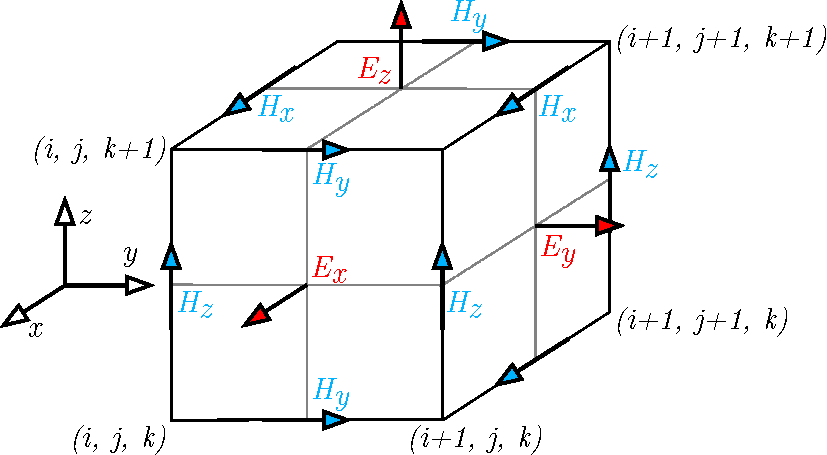
\includegraphics[width=.95\textwidth]{yee lattice.pdf}
            \end{figure}
        \end{column}%
    \end{columns}
    \begin{outline}
        \1 We are going to compute \textit{only one} component at a given point
        \1 There are no field components at the lattice edges
        \1 Each component is similarly spaced.
    \end{outline}
\end{frame}


\begin{frame}
    \frametitle{The Yee Algorithm}
    \begin{outline}
        \1 Developed in 1966 by Kane Yee
        \1 The algorithm employs second-order ($O(\Delta^2)$) central differences.
    \end{outline}
    \begin{outline}[enumerate]
        \1 Replace all the derivatives in Ampere's and Faraday's laws with finite differences.

        \2 Discretize space and time so that the electric and magnetic fields are staggered in both space and time.
        \1 Evaluate the magnetic fields one time-step into the future ($n+1$)
        \1 Evaluate the electric fields into the future ($n +  1$)
        \1 Repeat Steps 2 and 3 until all the fields have been computed.
    \end{outline}
\end{frame}

\begin{frame}
    \frametitle{Online Notebook}
    \begin{outline}
        \1 Google Colab notebook running a Python example
        \1 We focus on 1D FDTD first.
        \1 Alternatively, download the Python repository from:
    \end{outline}
    \begin{figure}[h!]
        \centering
        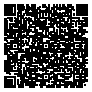
\includegraphics[width=.45\textwidth]{qrcode.pdf}
    \end{figure}
\end{frame}

\begin{frame}
    \frametitle{The Yee Algorithm in 1D}
    Let's write the time-dependent Maxwell's equations that have the curl operations:
    \begin{align*}
        \pdv{\va{E}}{t} & = \frac{1}{\E_0} \curl{\va{H}}  \\
        \pdv{\va{H}}{t} & = -\frac{1}{\u_0} \curl{\va{E}}
    \end{align*}
    For one-dimensional case, we have:
    \begin{align*}
        \pdv{{E_z}}{t} & = \frac{1}{\E_0} \pdv{H_y}{x}  \\
        \pdv{{H_y}}{t} & = -\frac{1}{\u_0} \pdv{E_z}{x}
    \end{align*}


\end{frame}

\begin{frame}
    \frametitle{The Yee Algorithm in 1D}
    We will be using the finite difference notation to express the fields and derivatives (differences)
    \begin{align*}
        E_{z}(x, t)=E_{z}\left(i \Delta_{x}, n \Delta_{t}\right)=E_{z}^{n}[i] \\
        H_{y}(x, t)=H_{y}\left(i \Delta_{x}, n \Delta_{t}\right)=H_{y}^{n}[i]
    \end{align*}
    Here $\Delta_x$ and $\Delta_t$ are offsets in space and time. Indices $i$ and $n$ represent steps in space and time.

    The 1D Maxwell's (Faraday's) equations then become:
    \begin{equation*}
        \left.\u \pdv{H_y}{t}
        \right|_{(i+1/2)\Delta_x,n\Delta_t}
        =
        \left.\pdv{E_z}{x}\right|_{(i+1/2)\Delta_x,n\Delta_t}
        \label{eq:faradayDiscrete}
    \end{equation*}
    \begin{equation*}
        \u\frac{H_y^{n+\frac{1}{2}}\left[i+\frac{1}{2}\right] -
        H_y^{n-\frac{1}{2}} \left[i+\frac{1}{2}\right]} {\Delta_t} =
        \frac{E_z^{n} \left[i+1\right] - E_z^{n} \left[i\right]}{\Delta_x}
        \label{eq:faradayFdtd1D}
    \end{equation*}
\end{frame}

\begin{frame}[fragile]
    \frametitle{The Yee Algorithm in 1D - Faraday's Law}

    \begin{figure}[h!]
        \centering
        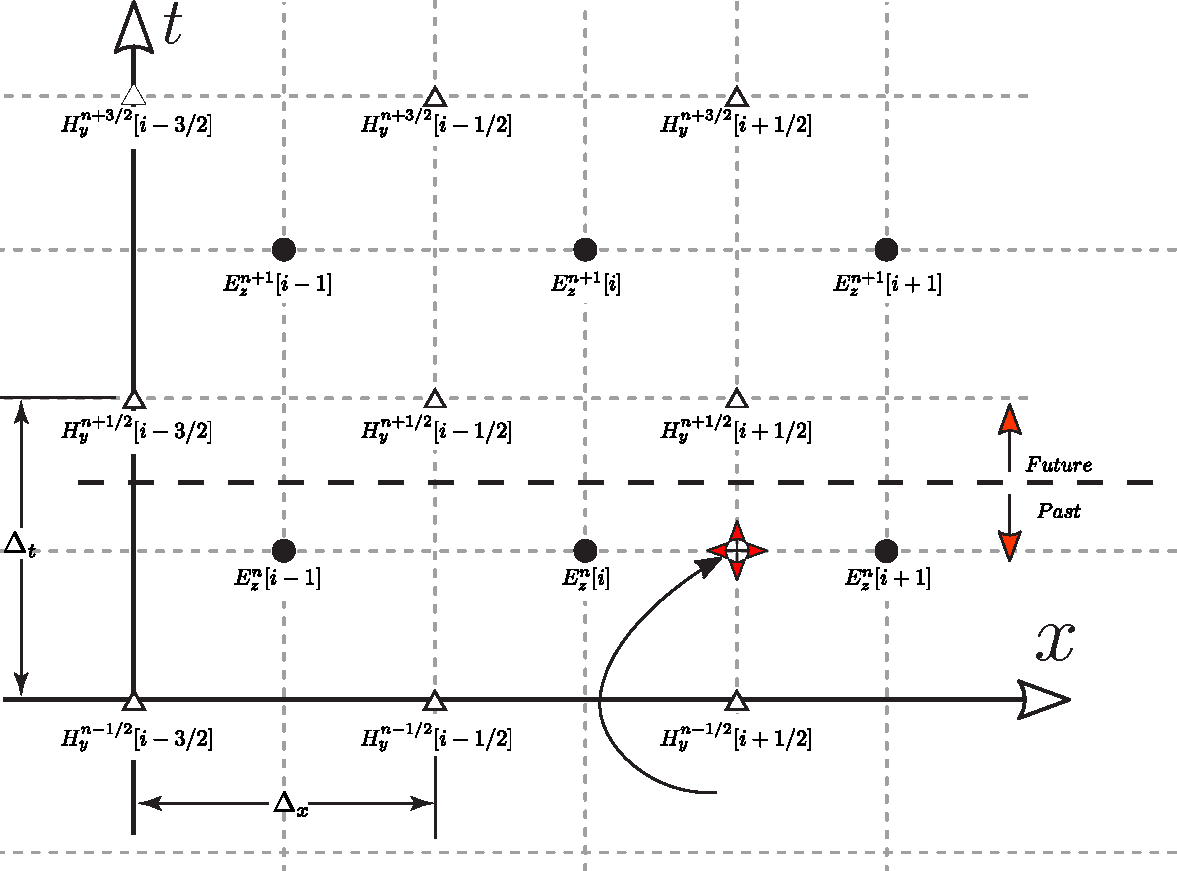
\includegraphics[width=.6\textwidth]{space_time marching.pdf}
        \caption{The interleaved $E_z$ and $H_y$ points in space and time.}
    \end{figure}

    \begin{equation}
        H_y^{n+\frac{1}{2}}\left[i+\frac{1}{2}\right] = H_y^{n-\frac{1}{2}}\left[i+\frac{1}{2}\right] +
        \frac{\Delta_t}{\mu\Delta_x}
        \left(E_z^{n}\left[i+1\right] - E_z^{n}\left[i\right]\right).
        \label{eq:updateHy}
    \end{equation}

\end{frame}


\begin{frame}
    \frametitle{The Yee Algorithm in 1D - Ampere's Law}
    Using similar techniques, we get the update equation for the electric field using the Ampere's law:
    \begin{equation}
        E_z^{n+1}\left[i\right] = E_z^{n}\left[i\right] +
        \frac{\Delta_t}{\E\Delta_x}
        \left(H_y^{n+\frac{1}{2}}\left[i+\frac{1}{2}\right] - H_y^{n+\frac{1}{2}}\left[i-\frac{1}{2}\right]\right).
    \end{equation}

\end{frame}

\begin{frame}
    \frametitle{The Courant Number}
    \begin{outline}
        \1 We have the update coefficients $\frac{\Delta_t}{\E\Delta_x}$ and $\frac{\Delta_t}{\u\Delta_x}$  in the electric and magnetic fields expressions.
        \1 These coefficients determine how far the energy propagates in a single step in time and space.
        \1 Knowing $c = 1/\sqrt{\E_0 \u_0}$, the maximum distance energy can travel in \textit{one} time step is $c \Delta_t$
        \1 Courant number $S_c$ is the ratio $c \Delta_t / \Delta_x$
        \2 It determines the stability of the simulation.
    \end{outline}

    \begin{align*}
        \frac{1}{\E} \frac{\Delta_{t}}{\Delta_{x}} & =\frac{1}{\E_{r} \E_{0}} \frac{\sqrt{\E_{0} \u_{0}}}{\sqrt{\E_{0} \u_{0}}} \frac{\Delta_{t}}{\Delta_{x}}=\frac{\sqrt{\E_{0} \u_{0}}}{\E_{r} \E_{0}} \frac{c \Delta_{t}}{\Delta_{x}}=\frac{1}{\E_{r}} \sqrt{\frac{\u_{0}}{\E_{0}}} \frac{c \Delta_{t}}{\Delta_{x}}=\frac{\eta_{0}}{\E_{r}} \frac{c \Delta_{t}}{\Delta_{x}}=\frac{\eta_{0}}{\E_{r}} S_{c}      \\
        \frac{1}{\u} \frac{\Delta_{t}}{\Delta_{x}} & = \frac{1}{\u_{r} \u_{0}} \frac{\sqrt{\E_{0} \u_{0}}}{\sqrt{\E_{0} \u_{0}}} \frac{\Delta_{t}}{\Delta_{x}}=\frac{\sqrt{\E_{0} \u_{0}}}{\u_{r} \u_{0}} \frac{c \Delta_{t}}{\Delta_{x}}=\frac{1}{\u_{r}} \sqrt{\frac{\E_{0}}{\u_{0}}} \frac{c \Delta_{t}}{\Delta_{x}}=\frac{1}{\u_{r} \eta_{0}} \frac{c \Delta_{t}}{\Delta_{x}}=\frac{1}{\u_{r} \eta_{0}} S_{c}
    \end{align*}
\end{frame}



\begin{frame}[fragile]
    \frametitle{Final Expressions}
    \begin{figure}[h!]
        \centering
        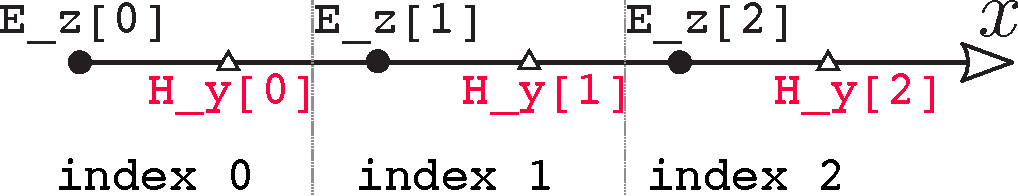
\includegraphics[width=.7\textwidth]{code_fdtd_1d.pdf}
        \caption{Array variable definition for 1D FDTD.}
    \end{figure}
    The update equations for a computer program therefore are:
    \begin{minted}{python}
    hy[i] = hy[i] + (ez[i + 1] - ez[i]) / imp0

    ez[i] = ez[i] + (hy[i] - hy[i - 1]) * imp0
\end{minted}
    Here \texttt{imp0} is the characteristic impedance, and $S_c = 1$ is assumed 1. Note the magnetic field is calculated first and then the electric field. We place the expressions above in a loop.
\end{frame}


\begin{frame}
    \frametitle{Some Important Observations}

    \begin{outline}
        \1 The points at the boundary need to be dealt with differently. As an example,
        for \texttt{ez[0]}, we dont have        \texttt{hy[-1]}.
        \2 Similarly, for \texttt{hy[MAX-1]}, there is no \texttt{ez[MAX]}
        \2 \textcolor{red}{We can apply absorbing boundary conditions}
        \1 Only having one impedance results in a homogeneous medium
        \2 \textcolor{red}{We can assign each node a $\E$ and $\u$}
        \1 Right now we haven't talked about introducing energy into the system
        \2 \textcolor{red}{We can create a hard-wired source}
    \end{outline}

\end{frame}

\begin{frame}[fragile]
    \frametitle{A Simple Python 1D FDTD Simulation}
    \scriptsize
    \begin{minted}{python}

# do time stepping
for n in range(maxTime):

# update magnetic field
for i in range(SIZE-1):
hy[i] = hy[i] + (ez[i + 1] - ez[i]) / imp0

# update electric field
for i in range(SIZE):
ez[i] = ez[i] + (hy[i] - hy[i - 1]) * imp0

# Additive Gaussian source node */
if n < sourceSigma:
    ez[0] = math.exp(-((n - 1*sourcePeakTime)/)**2 / sourceSigma)
else:
    ## PEC Boundaries
    ez[0] = 0.0
    ez[(SIZE - 1)] = 0.0

print(ez[sensorLocation])
#done with time stepping loop
    \end{minted}

\end{frame}

\begin{frame}[fragile]
    \frametitle{Modelling Open Space}
    \frametitle{Plotting Impedance}
    \begin{columns}[T] % align columns
        \begin{column}{.4\textwidth}

            To simulate infinite space, we use special types of boundary conditions called absorbing boundary conditions (ABCs).

            \textcolor{red}{ABCs are approximate and introduce dispersion especially in higher dimensions}

            Simple ABC's are:
            \begin{minted}[]{python}
    ez[0] = ez[1] 
    hy[MAX-1] = hy[MAX-2]
\end{minted}
        \end{column}
        \begin{column}[T]{.6\textwidth}
            \begin{figure}
                \centering
                \includegraphics[width=.8\textwidth]{chamber.jpeg}
                \caption{F-16 inside an RF anechoic test chamber.}
            \end{figure}
        \end{column}%
    \end{columns}

\end{frame}

\begin{frame}[fragile]
    \frametitle{Modelling Sources}

    \begin{outline}
        \1  In FDTD, we can either use \textit{hard-wired} sources or \textit{additive sources}.
        \1 The former is easier to implement but suffers from severe discontinuity on the point of generation
        \1 The latter just introduces a current term in the electric field update equation.
    \end{outline}

    \scriptsize
    \begin{minted}{python}
            
if n < sourceSigma:
    ez[0] = math.exp(-(n - sourcePeakTime)**2 / sourceSigma)
else:
    ez[0] = 0.0
            \end{minted}
    \centering
    Hardwired source
    \scriptsize
    \begin{minted}{python}
            
ez[50] += math.exp(-(n - sourcePeakTime)**2 / sourceSigma)
            \end{minted}
    \centering
    Additive Source

\end{frame}

\begin{frame}[fragile]
    \frametitle{Introducing Materials}
 Recall we have the material coefficients in the electric and magnetic field update equations:
 \begin{align*}
    H_y^{n+\frac{1}{2}}\left[i+\frac{1}{2}\right] = H_y^{n-\frac{1}{2}}\left[i+\frac{1}{2}\right] +
    \frac{\Delta_t}{\u\Delta_x}
    \left(E_z^{n}\left[i+1\right] - E_z^{n}\left[i\right]\right) \\
    E_z^{n+1}\left[i\right] = E_z^{n}\left[i\right] +
    \frac{\Delta_t}{\E\Delta_x}
    \left(H_y^{n+\frac{1}{2}}\left[i+\frac{1}{2}\right] - H_y^{n+\frac{1}{2}}\left[i-\frac{1}{2}\right]\right)
 \end{align*}
    We can therefore define $\E$ and $\u$ at any point in the FDTD simulation:
    \begin{minted}{python}
hy[i] = hy[i] + (ez[i + 1] - ez[i]) / imp0 / muR[i]
ez[i] = ez[i] + (hy[i] - hy[i - 1]) * imp0 / epsR[i]
    \end{minted}

\end{frame}

\begin{frame}
    \frametitle{Further Reading}

    Chapters 2 \& 3 — Understanding the FDTD Method \footcite{schneider_understanding_nodate}
  


\end{frame}

%% example of an ANIMATED FRAME
% \begin{frame}

%         \begin{animateinline}[autoplay]{20}
%             \multiframe{21}{rXmax=0+0.1}{
%               \begin{tikzpicture}
%               \begin{axis}[
%                 axis lines=center,
%                 domain=0.001:\rXmax,
%                 xtick={0,1,...,8},
%                 xmax=8.4,
%                 ymax=1.6,
%                 samples=51
%               ]
%               \addplot [gray, dashed] {1};

%               \addplot [color=red] {1-exp(-x)*cos(3*deg(x))};

%               \end{axis}
%               \end{tikzpicture}
%             }
%             \end{animateinline}

%   \end{frame}


\end{document}
